%%%%%%%%%%%%%%%%%%%%%%%%%%%%%%%%%%%%%%%%%%%%%%%%%%%%%%%%%%%%%%%%%%%%%%%%%%%%%
%% Original default rstudio/pandoc latex file
%% upated by @jhollist 09/15/2014
%% inspired by @cboetting https://github.com/cboettig/template and
%% @rmflight blog posts:
%% http://rmflight.github.io/posts/2014/07/analyses_as_packages.html 
%% http://rmflight.github.io/posts/2014/07/vignetteAnalysis.html).  
%%%%%%%%%%%%%%%%%%%%%%%%%%%%%%%%%%%%%%%%%%%%%%%%%%%%%%%%%%%%%%%%%%%%%%%%%%%%%

\documentclass[11pt,]{article}
\usepackage[T1]{fontenc}
\usepackage{lmodern}
\usepackage{amssymb,amsmath}
\usepackage{ifxetex,ifluatex}
\usepackage{fixltx2e} % provides \textsubscript
% use upquote if available, for straight quotes in verbatim environments
\IfFileExists{upquote.sty}{\usepackage{upquote}}{}
\ifnum 0\ifxetex 1\fi\ifluatex 1\fi=0 % if pdftex
  \usepackage[utf8]{inputenc}
\else % if luatex or xelatex
  \ifxetex
    \usepackage{mathspec}
    \usepackage{xltxtra,xunicode}
  \else
    \usepackage{fontspec}
  \fi
  \defaultfontfeatures{Mapping=tex-text,Scale=MatchLowercase}
  \newcommand{\euro}{€}
\fi
% use microtype if available
\IfFileExists{microtype.sty}{\usepackage{microtype}}{}
\usepackage[margin=1in]{geometry}
\usepackage{graphicx}
% Redefine \includegraphics so that, unless explicit options are
% given, the image width will not exceed the width of the page.
% Images get their normal width if they fit onto the page, but
% are scaled down if they would overflow the margins.
\makeatletter
\def\ScaleIfNeeded{%
  \ifdim\Gin@nat@width>\linewidth
    \linewidth
  \else
    \Gin@nat@width
  \fi
}
\makeatother
\let\Oldincludegraphics\includegraphics
{%
 \catcode`\@=11\relax%
 \gdef\includegraphics{\@ifnextchar[{\Oldincludegraphics}{\Oldincludegraphics[width=\ScaleIfNeeded]}}%
}%
\ifxetex
  \usepackage[setpagesize=false, % page size defined by xetex
              unicode=false, % unicode breaks when used with xetex
              xetex]{hyperref}
\else
  \usepackage[unicode=true]{hyperref}
\fi
\hypersetup{breaklinks=true,
            bookmarks=true,
            pdfauthor={},
            pdftitle={Combined effects of protein expression variance and correlation on multicomponent systems},
            colorlinks=true,
            citecolor=blue,
            urlcolor=blue,
            linkcolor=magenta,
            pdfborder={0 0 0}}
\urlstyle{same}  % don't use monospace font for urls
\setlength{\parindent}{0pt}
\setlength{\parskip}{6pt plus 2pt minus 1pt}
\setlength{\emergencystretch}{3em}  % prevent overfull lines
\setcounter{secnumdepth}{0}

%%%%%%%%%%%%%%%%%%%%%%%%%%%%%%%%%%%%%%%%%%%%%%%%%%%%%%%%
%Changes borrowed from @cboettig, added by @jhollist 
% A modified page layout 
\textwidth 6.75in
\oddsidemargin -0.15in
\evensidemargin -0.15in
\textheight 9in
\topmargin -0.5in
\usepackage{lineno} % add 
%%%%%%%%%%%%%%%%%%%%%%%%%%%%%%%%%%%%%%%%%%%%%%%%%%%%%%%%

%%%%%%%%%%%%%%%%%%%%%%%%%%%%%%%%%%%%%%%%%%%%%%%%%%%%%%%%
%%Packages and layout changes by @jhollist 09/15/2014
\usepackage{ragged2e}
\usepackage[font=normalsize]{caption}
  \usepackage[doublespacing]{setspace}
\usepackage{parskip}
\usepackage{fancyhdr}
\pagestyle{fancy}
\fancyhf{}
\renewcommand{\headrulewidth}{0pt}
\lfoot{\thepage}
%%Changed default abstract width and added lines
\renewenvironment{abstract}{
  \hfill\begin{minipage}{1\textwidth}
  \rule{\textwidth}{1pt}\vspace{5pt}
  \normalsize
  \begin{justify}
  \bfseries\abstractname\vspace{5pt}
  \end{justify}}
  {\par\noindent\rule{\textwidth}{1pt}\end{minipage}
}
%%%%%%%%%%%%%%%%%%%%%%%%%%%%%%%%%%%%%%%%%%%%%%%%%%%%%%%%

\title{Combined effects of protein expression variance and correlation on
multicomponent systems}
\author{
Kyle M. Kovary
Mary N. Teruel
}
\date{}
% Allowing for landscape pages
\usepackage{lscape}
\newcommand{\blandscape}{\begin{landscape}}
\newcommand{\elandscape}{\end{landscape}}

% Left justification of the text: see https://www.sharelatex.com/learn/Text_alignment
% \usepackage[document]{ragged2e} % already in the latex template
\newcommand{\bleft}{\begin{flushleft}}
\newcommand{\eleft}{\end{flushleft}}

%%Fix tightlist error: https://stackoverflow.com/questions/40438037/tightlist-error-using-pandoc-with-markdown
%%Added 2018-03-26 
\providecommand{\tightlist}{%
  \setlength{\itemsep}{0pt}\setlength{\parskip}{0pt}}
%%%  
  

\begin{document}
%%Edited by @jhollist 09/15/2014
%%Adds title from YAML
\begin{singlespace}
\begin{center}
\huge Combined effects of protein expression variance and correlation on
multicomponent systems
\end{center}
%%Adds Author, correspond email asterisk, and affilnum from YAML
\begin{center}
\large
Kyle M. Kovary \textsuperscript{1} 
Mary N. Teruel \textsuperscript{1} 
\end{center}
%%Adds affiliations from YAML
\begin{justify}
\footnotesize \emph{ 
\\*
\textsuperscript{1}Department of Chemical and Systems Biology, Stanford University,
Stanford, CA 94305, USA.\\*
}
%%Adds corresponding author email(s) from YAML
\newcounter{num}
\setcounter{num}{1}
\\[0.1cm]
\footnotesize \emph{ 
}
\end{justify}
%%Adds date from YAML
\normalsize

\begin{abstract}
Protein expression variation leads to phenotypic variance between cells.
This has been demonstrated in cell signaling and differentiation
decisions. Additionally coordinated expression of proteins between cells
can tune signaling pathways either towards a more binary or analog
modality. Though there is some evidence in bulk cell measurements and in
bacteria that certain heteromeric subunits or metabolic pathways may be
expressed in a coordinated fashion (i.e.~operons in bacteria), there has
not been a direct measurement of coordinated expression of proteins
(independent of TFs) in metazoans (vertebrates?). Here, we measure
cell-to-cell variability of relative protein abundance using
quantitative proteomics of individual \emph{Xenopus laevis} eggs and
show that proteins involved in metabolic pathways or members of
heteromeric complexes tend to have high correlations with other members
of those pathways/complexes. Our previous work highlighted the fact that
correlated expression increases the total variation of a pathway, so one
would reason that certain pathways or complexes would need to compensate
of this extra source of by reducing the variation of expression of these
pathways or complexes. To test this we computed total variance score
that took into account both the coefficient of variance and correlations
between proteins in a pathway and found that the lower 10\% of GO terms
were highly enriched for metabolic pathways. When we looked at the
relationship between CV and R between these GO terms we found a negative
relationship between them, demonstrating that increased correlation
needs to come at the expense of decreased variance. Simple molecular
models of heteromeric complexes and metabolic pathways demonstrate that
this tradeoff can result in higher efficiencies in both function and
reduced energy waste. Together, our study argues for a control principle
whereby coordinated expression of proteins in a pathway can require
lower variance in order to reduce the overall pathway variance, enabling
accurate control of active complexes or metabolic pathway activity.
\end{abstract}
\end{singlespace}


\emph{Keywords}: single cell, proteomics, stochasticity

\doublespace

\bleft

\justify

\hypertarget{introduction}{%
\section{Introduction}\label{introduction}}

The coordinated expression of proteins is vital for many aspects of
cellular function, from maintaining a dynamic steady state to
differentiation of cells into specialized types in different tissues.
The ability to regulate coordinated expression has been demonstrated to
occur via transcription (transcription factors, chromatin regulation),
translation (specialized ribosomes, mRNA structure/modifications), and
degradation (E3 ligases). These processes, as well as the molecules they
target, are all subject to noise, which has been shown to lead to
differences in cell behavior and decisions in otherwise identical cells.
Variability and coordinated expression (correlation) of proteins leads
to increased population level control in binary decisions, and a
decreased ability to execute analog signaling.

Despite these important insights, a global understanding of the
variability of protein expression between single cells and the
coordinated expression of groups of proteins is largely an nonexistent.
To systematically assess these properties of single cells, we carried
out a proteomics experiment on exceeding large single cells, Xenopus
laevis eggs. An advantage of this approach is that we can get around
much of the signal to noise issues that accompany studying single cells
due to low sample amounts. Additionally, at this stage of development
transcription is restricted so we are able to gain insights into
non-transcriptional control of protein expression. We also utilized
isobaric tagging in order to measure 25 individual eggs in 5 mass
spectrometry runs. In this study, we were able to measure the relative
abundance \textgreater{}1000 proteins across single cells in order to
better understand the properties of stochastic and coordinated
expression of proteins.

With this dataset we have been able to, for the first time, measured the
relationship between protein expression variance and coordinated protein
expression on a proteome scale in single cells. We have observed that
certain classes of proteins, including protein complexes and metabolic
pathways, are expressed in such a way that increased coordinated
expression is balanced by decreased variation. By doing this, cells are
able to decrease the total variance of a given complex or pathway, an
elegant balancing act that allows for finer control of metabolic
throughput and controlling the number of potentially formed complexes
though stoichiometric control. Though this kind of coordinated
expression leads to an increase in variance in a population of cells, it
can reduce variation within a cell.

\hypertarget{results}{%
\section{Results}\label{results}}

\hypertarget{single-cell-proteomics-reveals-global-protein-expression-variability-and-coordinated-expression-between-protein-pairs.}{%
\subsection{Single cell proteomics reveals global protein expression
variability and coordinated expression between protein
pairs.}\label{single-cell-proteomics-reveals-global-protein-expression-variability-and-coordinated-expression-between-protein-pairs.}}

The specific requirments for coordinated protein expression of pathways
or complexes can vary, with some requiring strict stoichiometric
regulation with others having much more relaxed requirements. Strict
stoichiometry scenerios require coordinated expression of proteins
(Figure 1A, top), and others can have uncoordinated expression (Figure
1A bottom). At the single cell level, coordinated expression will result
in a high correlation coefficient, whereas un-coordinated expression
will result in a low correlation coefficient (Figure 1B). Even when the
expression variation (standard deviation or coefficient of variation)
and abundance is identical between these two scenerios, the total
variance of a pathway or complex can be significantly different due to
the variance sum law:
\(var\left(\sum_{i=1}^n X_{i}\right) = \sum_{i=1}^{n} var(X_{i}) + 2\sum_{i,j:i<j}^{n} cov(X_{i},X_{j})\)
(Figure 1C). Our previous work has shown that this effect is important
in single cell pathway activation dynamics (Kovary et al., 2018).

In order to study the relationship between protein expression variance
and coexpression (correlated expression) of cellular pathways and
complexes at the proteome level, we utilized \emph{Xenopus laevis} eggs
as a single cell model. Activated \emph{Xenopus laevis} eggs were
collected at 5 time points across the first cell cycle (0, 20, 40, 60,
and 80 minutes), with 5 eggs at each time point. Using TMT multiplexing
and mass spectrometry, we were able to determine the relative abundance
of more than 1300 proteins. Expression of these proteins were largely
invariant across the cell cycle, revealing that these highly expressed
genes are likely not regulated by cell cycle processes. Additionally, a
PCA analysis of these eggs showed no discernible clustering on cell
cycle time (Fig S1).

To determine the variance across these proteins, we calculated the
variance and coefficient of variation (CV) using all time points
collected. This showed a wide range of variation containing multiple
distributions (Fig 1D), many of which are consistent with our previous
study of variation using targeted mass spectrometry (Fig S2). In order
to see if variation was a regulated process, we grouped the protein
variation by gene ontology terms (GO terms) and plotted them in ranked
order. We saw that in general, processes xxx were\ldots{}

Since we were able to measure all of these proteins within single cells,
we are able to calculate coordinated expression of protein pairs at
single cell resolution. Using Pearson correlation coefficient, we could
determine coordinated expression of nearly 2 million protein pairs (Fig
1C) The distribution of correlation coefficients fit a normal
distribution, with the majority of protein pairs appearing to not show
significant coregulation. However, there appear to be a significant
number of protein pairs containing high correlation coefficients, and
the heatmap showed a lot of clustering of these highly coregulated pairs
(Fig 1D).

\begin{figure}
\centering
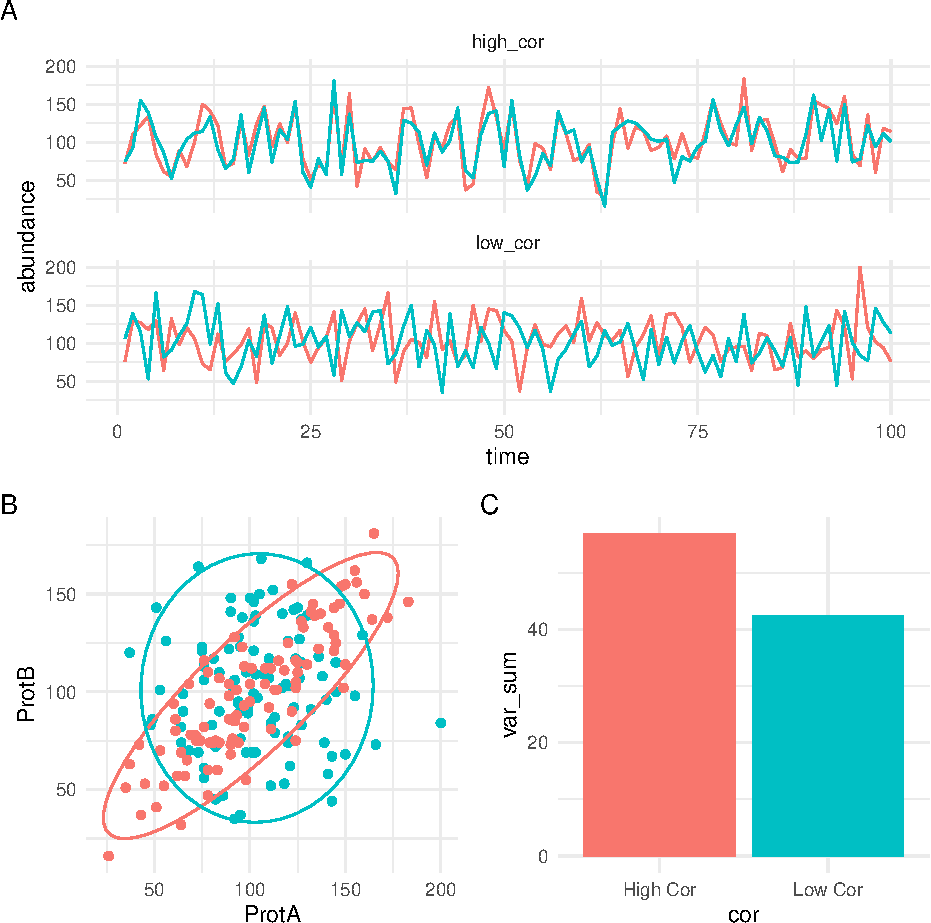
\includegraphics{output/figures/figure_1-1.pdf}
\caption{A) Simulated expression of two proteins over time in a single
cell with a mean of 100 and a standard deviation of 30 with expression
correlations of 0 and 0.8. B) Pairwise plots of the two proteins in the
single cells between uncorrelated and correlated scenerios. C) The total
variance between the uncorrelated and correlated scenerios from A and
B.}
\end{figure}

\hypertarget{protein-modules-display-different-levels-of-regulation-of-noise-and-co-expression-of-constituents}{%
\subsection{Protein modules display different levels of regulation of
noise and co-expression of
constituents}\label{protein-modules-display-different-levels-of-regulation-of-noise-and-co-expression-of-constituents}}

To investigate whether coordinated expression goes beyond just protein
pairs, we wanted to see if pathways, complexes, and other modules had
proteins that with coordinated expression. To answer this question, we
grouped proteins by GO terms and calculated the median correlation
coefficient across all pairs of proteins within the term. When the
ranked media correlation is plotted it's clear that there are a
significant number of GO terms with higher than expected levels of
coordinate expression.

\hypertarget{total-variance-metric-reveals-certain-modules-enforce-a-tradeoff-between-protein-co-expression-and-noise}{%
\subsection{Total variance metric reveals certain modules enforce a
tradeoff between protein co-expression and
noise}\label{total-variance-metric-reveals-certain-modules-enforce-a-tradeoff-between-protein-co-expression-and-noise}}

Variance Sum Law --- Dependent Case

The sum of variance for a group of proteins \(X_{1},\dotsc,X_{n}\) with
dependent relationships:

\[\sigma_{{}_{total}} = \sqrt{var\left(\sum_{i=1}^n X_{i}\right)}\]

\[\sigma_{{}_{norm}} = \dfrac{\sigma_{{}_{total}}}{n}\]

When calculating the total variance of a pathway or general group of
proteins, the total variance is the square root of the sums of the
squares of the coefficient of variance. However, if any of the proteins
are correlated in expression, an extra term must be added to account for
this correlation. This means that if a group of proteins have a positive
correlation, then the total variance will be higher than if there was no
correlation. In order to study how variance and coordinated expression
are related between single cells, we wanted to calculate a normalized
total variance metric. Since we were not interested in the increase of
variance due to the number of proteins in a module, we calculated the
total variance using the coefficient of variation and correlation
coefficients and normalize to the total number of proteins in the
module. When total variance is plotted against the number of proteins,
there is a clear linear relationship between the two. Once we normalize
to the total number of proteins this relationship is lost and we are
left with the effects of coefficient of variation and correlation.

\hypertarget{low-total-variance-modules-are-enriched-for-metabolic-pathways-and-heteromeric-protein-complexes}{%
\subsection{Low total variance modules are enriched for metabolic
pathways and heteromeric protein
complexes}\label{low-total-variance-modules-are-enriched-for-metabolic-pathways-and-heteromeric-protein-complexes}}

\hypertarget{enforcement-of-a-tradeoff-between-protein-co-expression-and-noise-increases-efficiency-of-metabolic-pathways-and-heteromeric-protein-complexes}{%
\subsection{Enforcement of a tradeoff between protein co-expression and
noise increases efficiency of metabolic pathways and heteromeric protein
complexes}\label{enforcement-of-a-tradeoff-between-protein-co-expression-and-noise-increases-efficiency-of-metabolic-pathways-and-heteromeric-protein-complexes}}

\hypertarget{methods}{%
\section{Methods}\label{methods}}

\hypertarget{collection-and-activation-of-xenopus-laevis-eggs}{%
\subsection{Collection and activation of Xenopus laevis
eggs:}\label{collection-and-activation-of-xenopus-laevis-eggs}}

Xenopus egg extracts were prepared based on modifications of a previous
protocol (Tsai et al, 2014). All of the animal protocols used in this
manuscript were approved by the Stanford University Administrative Panel
on Laboratory Animal Care. To induce egg laying, female Xenopus laevis
were injected with human chorionic gonadotropin injection the night
before each experiment. To collect the eggs, the frogs were subjected to
pelvic massage, and the eggs were collected in 1X Marc's Modified
Ringer's (MMR) buffer (0.1 M NaCl, 2 mM KCl, 1 mM MgCl2, 2 mM CaCl2, 5
mM HEPES, pH 7.8). To remove the jelly coat from the eggs, they were
placed in a solution of 2\% cysteine in 1× MMR buffer for 4 min and
gently agitated, after which they were washed four times with 1× MMR
buffer. To activate the cell cycle, eggs were placed in a solution of
0.5 \(\mu\)g/ml of calcium ionophore A23187 (Sigma) and 1X MMR buffer
for 3 min, after which they were washed four times with 1× MMR buffer.
Single eggs were collected at their respective timepoints and placed
into 600uL tubes and snap frozen in liquid nitrogen before being stored
at 80°C.

\hypertarget{sample-preparation-for-mass-spectrometry}{%
\subsection{Sample preparation for mass
spectrometry:}\label{sample-preparation-for-mass-spectrometry}}

Single eggs were lysed mechanically by pipetting the egg in 100\(\mu\)L
of lysis buffer (100 mM NaCl, 25 mM Tris pH 8.2, Complete EDTA- free
protease inhibitor cocktail (Sigma). The lysate was then placed in a 400
uLnatural polyethylene microcentrifuge tube (E\&K Scientific \#485050)
and spun at 15,000 g in a right angle centrifuge (Beckman Microfuge E)
at 4°C for 5 min. The lipid layer was removed by using a razor blade to
cut the tube off just beneath it, and the cytoplasmic fraction was
pipetted into a 1.5-ml protein LoBind tube (Fisher Scientific
\#13-698-794), being careful to leave the yolk behind. To precipitate
the proteins from the cytoplasmic fraction, 1 ml of ice cold acetone was
added to each sample and placed at 20°C overnight. To collect
precipitated proteins, the samples were centrifuged at 18,000 g for 20
min at 4°C. Acetone was decanted, and the protein pellets were
resolubilized in 25\(\mu\)L of 8 M urea. To fully solubilize the protein
pellet, the samples were placed in a shaker for 1 h at room temperature.
The samples were then diluted to 2 M urea with 50 mM ammonium
bicarbonate to a 100\(\mu\)L volume, after which protein concentration
was measured in duplicate with a BCA assay by taking two 10\(\mu\)L
aliquots of each sample. The proteins in the remaining 80\(\mu\)L of
sample volume were reduced with 10 mM TCEP and incubated for 30 min at
37°C, then alkylated with 15 mM iodoacetamide and incubated in the dark
at room temperature.

Next, the samples were diluted to 1 M urea with 50 mM ammonium
bicarbonate. Trypsin (Promega \#V5113) was then added at a ratio of 10
ng trypsin per 1ug protein (no \textless{} 500 ng was added to a
sample). The trypsin digestion was carried out at 37°C for 12--16 h. To
stop the trypsin, formic acid (Fisher \#A117-50) was added at a ratio of
3\(\mu\)l per 100\(\mu\)l of sample to bring the pH down to \textless{}
3.

Peptides were cleaned up using an Oasis HLB uElution plate (Waters),
equilibrated, and washed with 0.04\% trifluoroacetic acid in water, and
eluted in 80\% acetonitrile with 0.2\% formic acid. All solutions used
are HPLC grade. Samples were then lyophilized. To remove any variance
produced by phosphorylated peptides, the samples were
phosphatase-treated. Peptides were resolubilized in 50\(\mu\)L of 1X
NEBuffer 3 (no BSA), and calf intestinal alkaline phosphatase (NEB
\#M0290S) was added at a ratio 0.25 units per lg of peptide and
incubated for 1 h at 37°C. The peptides were cleaned up again according
to steps described above. Peptides were resolubilized in 2\%
acetonitrile and 0.1\% formic acid before MS analysis.

\hypertarget{mass-spectrometry-data-collection}{%
\subsection{Mass spectrometry data
collection:}\label{mass-spectrometry-data-collection}}

Ask SUMS for details

\hypertarget{mass-spectrometry-data-analysis}{%
\subsection{Mass spectrometry data
analysis:}\label{mass-spectrometry-data-analysis}}

Ask SUMS for details

\hypertarget{data-processing}{%
\subsection{Data processing:}\label{data-processing}}

To minimize the effects of non-biological variance, a correction factor
was used to correct for these biases. First, each peptide was normalized
by the median across all of the samples. Second, the vector of all
peptides for each cell was divided by the median value across all
peptides. Before peptides were used to estimate protein abundance,
highly variable peptides needed to be filtered out. Peptides were
grouped by their master UniProt accession number, and all peptides whose
log transformed values were more than 2\(\sigma\) away from the mean
were discarded. Next, protein abundances were estimated by taking the
median normalized value for each peptide for a protein in each sample.
Missing protein levels were imputed using the k-nearest neighbors
algorithm, with k being set to 1 and the similarity measure for distance
the Gower's distance between the proteome vectors.

\clearpage

\hypertarget{references}{%
\section{References}\label{references}}

\hypertarget{refs}{}
\leavevmode\hypertarget{ref-Kovary_2018}{}%
Kovary, K.M., Taylor, B., Zhao, M.L., and Teruel, M.N. (2018).
Expression variation and covariation impair analog and enable binary
signaling control. Molecular Systems Biology \emph{14}.

\eleft

\clearpage

\begin{verbatim}
R version 3.6.1 (2019-07-05)
Platform: x86_64-apple-darwin15.6.0 (64-bit)
Running under: macOS Catalina 10.15.3

Matrix products: default
BLAS:   /Library/Frameworks/R.framework/Versions/3.6/Resources/lib/libRblas.0.dylib
LAPACK: /Library/Frameworks/R.framework/Versions/3.6/Resources/lib/libRlapack.dylib

locale:
[1] en_US.UTF-8/en_US.UTF-8/en_US.UTF-8/C/en_US.UTF-8/en_US.UTF-8

attached base packages:
[1] stats     graphics  grDevices utils     datasets  methods   base     

other attached packages:
[1] knitcitations_1.0.10 knitr_1.28          

loaded via a namespace (and not attached):
 [1] Rcpp_1.0.3        lubridate_1.7.4   digest_0.6.24     plyr_1.8.5       
 [5] R6_2.4.1          jsonlite_1.6.1    formatR_1.7       magrittr_1.5     
 [9] evaluate_0.14     bibtex_0.4.2.2    httr_1.4.1        rlang_0.4.4      
[13] stringi_1.4.6     curl_4.3          xml2_1.2.2        rmarkdown_2.1    
[17] tools_3.6.1       stringr_1.4.0     RefManageR_1.2.12 xfun_0.12        
[21] yaml_2.2.1        compiler_3.6.1    htmltools_0.4.0  
\end{verbatim}

\end{document}